% ROZDZIAŁ 4 — plik włączany przez main.tex
\chapter{Miara Lebesgue'a na przestrzeni euklidesowej}
\label{ch:lebesgue}

\section{Co właściwie chcemy skonstruować?}

Długość przedziału $[a,b)$ to $b-a$, a objętość
$d$-wymiarowego prostopadłościanu
$Q=\prod_{j=1}^d[a_j,b_j)$ wynosi
$|Q|=\prod_{j=1}^d(b_j-a_j)$.
Chcemy rozciągnąć tę funkcję na bogatą rodzinę
podzbiorów $\mathbb R^d$, zachowując przeliczalną
addytywność i naturalną zgodność z geometrią.

Przy każdym $d\in\mathbb N$, $d\ge1$, przez
$\mathcal B(\mathbb R^d)$ oznaczamy $\sigma$-algebrę
borelowską z definicji \ref{def:borel}. Odróżniamy
\emph{miarę borelowską Lebesgue'a} $\lambda_d^B$
od jej uzupełnienia $\lambda_d$. Ich dziedziny nie są
jednakowe. Dla prostopadłościanów osiowych z dowolnym wyborem
otwartości i domknięcia ścian przez $|R|$ oznaczamy
\emph{elementarną objętość geometryczną}, czyli iloczyn
długości boków; nie zakładamy jeszcze, że jest ona miarą.
W szczególności dla $Q$ jest to wyjściowa objętość,
a dla zwartego $K$ lub otwartego $O$ ta sama liczba.
Symbol $|R|$ nie jest na tym etapie miarą dowolnego zbioru.

\section{Objętość elementarna i lemat o pokryciach}

\begin{definicja}[Prostopadłościan półotwarty]
\label{def:halfopen-box}
Przez prostopadłościan półotwarty rozumiemy zbiór
$Q=\prod_{j=1}^d[a_j,b_j)$, gdzie $a_j,b_j\in\mathbb R$,
$a_j<b_j$. Rodzinę takich \emph{ograniczonych} zbiorów
oraz zbioru pustego oznaczamy $\mathcal Q_d$.
Kładziemy $|\varnothing|=0$ i
$|Q|=\prod_{j=1}^d(b_j-a_j)$ dla niepustego $Q$.
\end{definicja}

Użycie przedziałów półotwartych nie jest kosmetyczne.
Dla $a<c<b$ mamy rozkład rozłączny
$[a,b)=[a,c)\sqcup[c,b)$. Analogicznie przecięcie
dwóch prostopadłościanów półotwartych jest
prostopadłościanem tego samego typu lub zbiorem pustym,
a różnica takich zbiorów jest skończoną sumą rozłączną
prostopadłościanów półotwartych.

\begin{lemat}[Skończony podział na siatkę]
\label{lem:rect-grid}
Niech $Q_1,\ldots,Q_N\in\mathcal Q_d$.
Istnieje skończona rodzina parami rozłącznych
prostopadłościanów półotwartych $P_1,\ldots,P_M$, taka że
każdy z $Q_i$ jest sumą pewnych $P_j$. W konsekwencji
można jednoznacznie określić na rodzinie $\mathcal R_d$
wszystkich skończonych sum zbiorów z $\mathcal Q_d$
funkcję $v$, przyjmując
$v(\bigsqcup_{i=1}^NQ_i)=\sum_{i=1}^N|Q_i|$
dla dowolnego rozłącznego przedstawienia.
Funkcja $v$ jest nieujemna i skończenie addytywna.
\end{lemat}

\begin{proof}
W każdej współrzędnej wypisujemy w porządku rosnącym
wszystkie końce przedziałów występujących w $Q_i$.
Sąsiednie końce wyznaczają przedziały półotwarte;
ich iloczyny kartezjańskie dają skończoną siatkę.
Każdy $Q_i$ składa się z całych komórek siatki.
Dla każdej komórki $P=\prod_j[c_j,e_j)$ jej objętość
to $\prod_j(e_j-c_j)$. Dodawanie objętości przy
podziale w jednej współrzędnej jest rozdzielnością
mnożenia względem dodawania; iterując po współrzędnych,
otrzymujemy $|Q_i|$ jako sumę objętości jej komórek.
Jeżeli ten sam zbiór ma dwa rozłączne przedstawienia,
wspólna siatka dla obu przedstawień pokazuje, że oba
sumowania dają tę samą liczbę. Tak samo dowodzi się
skończonej addytywności $v$.
\end{proof}

\begin{uwaga}
$\mathcal R_d$ jest pierścieniem zbiorów, ale nie
algebrą podzbiorów $\mathbb R^d$, ponieważ
$\mathbb R^d\notin\mathcal R_d$. Na ograniczonym
prostopadłościanie $H$ rodzina
$\mathcal R_d|_H=\{A\cap H:A\in\mathcal R_d\}$
jest natomiast algebrą podzbiorów $H$.
To lokalne rozróżnienie pozwoli nam zastosować
rozdział \ref{ch:caratheodory} bez udawania, że
nieograniczona przestrzeń jest ograniczonym prostokątem.
\end{uwaga}

\begin{lemat}[Nierówność objętościowa dla pokryć]
\label{lem:rect-cover-ineq}
Jeżeli $Q,Q_1,Q_2,\ldots\in\mathcal Q_d$ i
$Q\subseteq\bigcup_{n\ge1}Q_n$, to
\begin{equation}\label{eq:rect-cover-volume}
|Q|\le\sum_{n=1}^\infty|Q_n|.
\end{equation}
\end{lemat}

\begin{proof}
Dla $Q=\varnothing$ twierdzenie jest oczywiste.
Niech $Q=\prod_j[a_j,b_j)$ będzie niepusty.
Wystarczy rozważyć przypadek, w którym suma po prawej
stronie jest skończona. Ustalmy $\varepsilon>0$ oraz
$0<\delta<\frac12\min_j(b_j-a_j)$ i połóżmy
$K_\delta=\prod_j[a_j+\delta,b_j-\delta]$.
Jest to zwarty podzbiór $Q$.

Każdy $Q_n$ można zawrzeć w otwartym prostopadłościanie
$O_n$ o objętości elementarnej mniejszej niż
$|Q_n|+\varepsilon2^{-n}$: wystarczy nieznacznie
przesunąć wszystkie jego ściany na zewnątrz.
Zbiory $O_n$ tworzą otwarte pokrycie $K_\delta$.
Ze zwartości istnieją $n_1,\ldots,n_N$ takie, że
$K_\delta\subseteq\bigcup_{i=1}^N O_{n_i}$.

Wykażmy osobno elementarną nierówność dla skończonego
pokrycia zwartego prostopadłościanu
$K=\prod_{j=1}^d[\alpha_j,\beta_j]$ przez otwarte
prostopadłościany $O_1,\ldots,O_m$:
$|K|\le\sum_{i=1}^m|O_i|$.
Dla dostatecznie małego $\eta>0$ wprowadzamy
$P_\eta=\prod_j[\alpha_j+\eta,\beta_j-\eta)$.
W każdej współrzędnej wybieramy wszystkie końce
przedziałów tworzących $O_i$ i $P_\eta$.
Skończona siatka złożona z tych punktów rozkłada
$P_\eta$ na parami rozłączne półotwarte komórki $S_l$.
Wnętrze komórki nie przecina żadnej hiperpłaszczyzny,
która jest ścianą $O_i$. Wybierzmy
$x_l\in\operatorname{int}S_l\subseteq K$.
Punkt $x_l$ należy do pewnego $O_{i(l)}$.
Ponieważ granice współrzędnych $O_{i(l)}$ należą do
siatki, wynika stąd
$\operatorname{int}S_l\subseteq O_{i(l)}$, a więc
$S_l\subseteq\overline{O_{i(l)}}$.

Dla ustalonego $i$ oznaczmy przez $\mathcal S_i$ rodzinę
komórek przypisanych do $O_i$. Niech $H_i^{(\gamma)}$
będzie półotwartym prostopadłościanem zawierającym
$\overline O_i$, którego długości boków przewyższają
odpowiednie długości $O_i$ o $2\gamma$.
Każda komórka $S_l\in\mathcal S_i$ jest zawarta w
$H_i^{(\gamma)}$. Na mocy skończonej addytywności
i monotoniczności elementarnej objętości na pierścieniu
$\mathcal R_d$ mamy
$\sum_{S_l\in\mathcal S_i}|S_l|
\le |H_i^{(\gamma)}|$.
Gdy $\gamma\downarrow0$, prawa strona dąży do $|O_i|$.
Komórki $S_l$ rozkładają $P_\eta$ i każdą przypisaliśmy
jednemu z $O_i$, zatem
\[
 |P_\eta|=\sum_l|S_l|
 =\sum_{i=1}^m\sum_{S_l\in\mathcal S_i}|S_l|
 \le\sum_{i=1}^m|O_i|.
\]
Wreszcie $|P_\eta|\to|K|$ przy $\eta\downarrow0$.
Argument ten wykorzystuje wyłącznie skończone podziały
prostopadłościanów i nie zakłada wcześniej istnienia miary
Lebesgue'a.
Stąd
\[
|K_\delta|\le\sum_{i=1}^N|O_{n_i}|
\le\sum_{n=1}^\infty|Q_n|+\varepsilon.
\]
Przy $\delta\downarrow0$ mamy
$|K_\delta|=\prod_j(b_j-a_j-2\delta)\to|Q|$.
Następnie $\varepsilon\downarrow0$, co dowodzi
\eqref{eq:rect-cover-volume}.
\end{proof}

\begin{uwaga}[W którym miejscu używamy zwartości?]
Bez zwartości nie mielibyśmy prawa zastąpić
przeliczalnego pokrycia skończonym i skorzystać
z rozkładu na siatkę. To zasadniczy krok geometryczny
w dowodzie, że elementarna objętość przechodzi
z addytywności skończonej do przeliczalnej.
\end{uwaga}

\begin{twierdzenie}[Premiara na ograniczonym prostopadłościanie]
\label{thm:volume-premeasure}
Dla ustalonego $H=\prod_{j=1}^d[a_j,b_j)\in\mathcal Q_d$
funkcja $v$ z lematu \ref{lem:rect-grid}, ograniczona do
algebry $\mathcal R_d|_H$, jest skończoną premiarą.
Jej przedłużenie na $\sigma(\mathcal R_d|_H)$ istnieje
i jest jednoznaczne.
\end{twierdzenie}

\begin{proof}
Wszystkie zbiory z $\mathcal R_d|_H$ są skończonymi
rozłącznymi sumami prostopadłościanów półotwartych
zawartych w $H$; wspólna siatka zapewnia skończoną
addytywność. W szczególności $v(H)=|H|<\infty$.

Niech $A=\bigsqcup_{n\ge1}A_n$, gdzie
$A,A_n\in\mathcal R_d|_H$. Z addytywności skończonej
i monotoniczności dostajemy
$\sum_{n=1}^Nv(A_n)\le v(A)$ dla każdego $N$, więc
$\sum_nv(A_n)\le v(A)$.
Rozbijmy $A$ i każdy $A_n$ na skończenie wiele
rozłącznych prostopadłościanów. Każdy składnik rozkładu
$A$ jest pokryty składnikami wszystkich $A_n$.
Lemat \ref{lem:rect-cover-ineq} daje po zsumowaniu
$v(A)\le\sum_nv(A_n)$. Zachodzi więc addytywność
przeliczalna w sensie definicji \ref{def:premeasure}.
Istnienie przedłużenia wynika z twierdzenia
\ref{thm:extension-caratheodory}, a jednoznaczność
z twierdzenia \ref{thm:extension-uniqueness}.
\end{proof}

\section{Konstrukcja miary Lebesgue'a}

\begin{definicja}[Miara zewnętrzna Lebesgue'a]
\label{def:lebesgue-outer}
Dla $E\subseteq\mathbb R^d$ określamy
\begin{equation}\label{eq:lebesgue-outer}
\lambda_d^*(E)=\inf\Big\{\sum_{n=1}^\infty|Q_n|:
Q_n\in\mathcal Q_d,\quad E\subseteq\bigcup_{n=1}^\infty Q_n\Big\}.
\end{equation}
Rodzinę zbiorów $\lambda_d^*$-mierzalnych w sensie
Carathéodory'ego oznaczamy $\mathcal L_d$.
Miarę $\lambda_d=\lambda_d^*|_{\mathcal L_d}$
nazywamy \emph{$d$-wymiarową miarą Lebesgue'a}.
\end{definicja}

\begin{twierdzenie}[Istnienie i podstawowe własności]
\label{thm:lebesgue-exists}
Dla każdego $d\ge1$ zachodzą następujące fakty:
\begin{enumerate}[label=\textup{(\roman*)}]
\item $\lambda_d^*$ jest miarą zewnętrzną;
\item każdy $Q\in\mathcal Q_d$ należy do $\mathcal L_d$ i
$\lambda_d(Q)=|Q|$;
\item $\mathcal B(\mathbb R^d)\subseteq\mathcal L_d$;
\item $\lambda_d$ jest zupełną i $\sigma$-skończoną miarą;
\item jej ograniczenie
$\lambda_d^B=\lambda_d|_{\mathcal B(\mathbb R^d)}$
jest jedyną miarą borelowską, która przypisuje każdemu
$Q\in\mathcal Q_d$ liczbę $|Q|$.
\end{enumerate}
\end{twierdzenie}

\begin{proof}
\emph{(i)} Rodzina $\mathcal Q_d$ zawiera $\varnothing$,
a $\mathbb R^d$ ma przeliczalne pokrycie prostopadłościanami
$[-n,n)^d$. Twierdzenie \ref{thm:outer-from-cover}
gwarantuje zatem, że \eqref{eq:lebesgue-outer}
określa miarę zewnętrzną.

\emph{(ii), równość objętości.}
Pokrycie $Q$ jednym $Q$ daje $\lambda_d^*(Q)\le|Q|$.
Lemat \ref{lem:rect-cover-ineq} daje nierówność
przeciwną dla każdego pokrycia dopuszczalnego w
\eqref{eq:lebesgue-outer}; zatem $\lambda_d^*(Q)=|Q|$.

\emph{(ii), mierzalność.}
Ustalmy $Q\in\mathcal Q_d$ i $T\subseteq\mathbb R^d$.
Dla każdego pokrycia $T\subseteq\bigcup_nR_n$, gdzie
$R_n\in\mathcal Q_d$, dzielimy $R_n$ wzdłuż ścian $Q$.
Przecięcie $R_n\cap Q$ jest jednym prostopadłościanem
półotwartym lub zbiorem pustym, natomiast
$R_n\setminus Q$ jest skończoną rozłączną sumą
takich prostopadłościanów. Na mocy lematu
\ref{lem:rect-grid} łączna objętość obu części wynosi
$|R_n|$. Części pierwszego rodzaju pokrywają
$T\cap Q$, a części drugiego $T\setminus Q$, więc
\[
\lambda_d^*(T\cap Q)+\lambda_d^*(T\setminus Q)
\le\sum_{n=1}^\infty |R_n|.
\]
Biorąc infimum po pokryciach, uzyskujemy nierówność
$\le\lambda_d^*(T)$; przeciwna jest zawsze prawdziwa.
Wynika stąd $Q\in\mathcal L_d$.

\emph{(iii)} Twierdzenie \ref{thm:caratheodory} daje,
że $\mathcal L_d$ jest $\sigma$-algebrą. Ponieważ zawiera
wszystkie prostopadłościany półotwarte, zawiera również
ich $\sigma$-algebrę, czyli $\mathcal B(\mathbb R^d)$
(twierdzenie \ref{thm:borel-Rd}).

\emph{(iv)} Zupełność daje twierdzenie
\ref{thm:caratheodory}. Dla $H_n=[-n,n)^d$ mamy
$\mathbb R^d=\bigcup_nH_n$ i
$\lambda_d(H_n)=(2n)^d<\infty$, więc miara jest
$\sigma$-skończona.

\emph{(v)} Niech $\nu$ będzie inną miarą borelowską
o zadanych wartościach na $\mathcal Q_d$.
Rodzina $\mathcal Q_d$ wraz z $\varnothing$ jest
układem $\pi$, generuje $\mathcal B(\mathbb R^d)$,
a rosnące prostopadłościany $H_n$ pokrywają całą
przestrzeń i mają tę samą skończoną miarę dla
$\nu$ oraz $\lambda_d^B$. Twierdzenie
\ref{thm:uniqueness-sigma-finite} daje
$\nu=\lambda_d^B$.
\end{proof}

\begin{uwaga}[Zgodność obu konstrukcji]
Dla każdego ograniczonego prostopadłościanu $H$
miara z twierdzenia \ref{thm:volume-premeasure} jest
równa ograniczeniu $\lambda_d^B$ do
$\mathcal B(H)$. Obie są skończonymi miarami na
tej samej $\sigma$-algebrze i zgadzają się na
półotwartych prostopadłościanach zawartych w $H$.
W ten sposób globalna konstrukcja przez pokrycia
zgadza się z lokalnym rozszerzaniem premiary.
\end{uwaga}

\section{Niezmienniczość względem przesunięć i skalowania}

\begin{lemat}[Zbiory zawarte w hiperpłaszczyźnie]
\label{lem:hyperplane-null}
Dla każdego $c\in\mathbb R$ i $1\le j\le d$
hiperpłaszczyzna $\{x\in\mathbb R^d:x_j=c\}$ ma
miarę Lebesgue'a zero. W szczególności każda skończona
lub przeliczalna rodzina punktów ma miarę zero.
\end{lemat}

\begin{proof}
Przecięcie hiperpłaszczyzny z $[-N,N)^d$ zawiera się
w półotwartym prostopadłościanie, którego $j$-ty bok
ma długość $2\delta$, a pozostałe długość $2N$
(po ewentualnym nieznacznym powiększeniu boków).
Z definicji miary zewnętrznej
$\lambda_d^*(\{x:x_j=c\}\cap[-N,N)^d)
\le (2N)^{d-1}2\delta$ dla dowolnego $\delta>0$.
Przechodząc z $\delta\downarrow0$, dostajemy wartość zero.
Hiperpłaszczyzna jest przeliczalną sumą takich przecięć,
a więc ma miarę zero. Singleton jest podzbiorem
hiperpłaszczyzny, a przeliczalna suma zbiorów zerowych
ma miarę zero na mocy \eqref{eq:subadditivity}.
\end{proof}

\begin{twierdzenie}[Translacje i jednolite skalowanie]
\label{thm:invariance-lebesgue}
Dla każdego $E\in\mathcal L_d$, każdego
$a\in\mathbb R^d$ i każdego $t\in\mathbb R\setminus\{0\}$
zbiory $a+E$ i $tE$ należą do $\mathcal L_d$ oraz
\begin{equation}\label{eq:lebesgue-invariance}
\lambda_d(a+E)=\lambda_d(E),\qquad
\lambda_d(tE)=|t|^d\lambda_d(E).
\end{equation}
Przyjmujemy tu $|t|^d\cdot\infty=\infty$.
\end{twierdzenie}

\begin{proof}
Udowodnimy najpierw mocniejszy fakt dotyczący miary
\emph{zewnętrznej}: dla każdego $E\subseteq\mathbb R^d$
zachodzi
$\lambda_d^*(a+E)=\lambda_d^*(E)$ oraz
$\lambda_d^*(tE)=|t|^d\lambda_d^*(E)$.

Dla translacji argument jest bezpośredni: jeśli
$E\subseteq\bigcup_nQ_n$, to
$a+E\subseteq\bigcup_n(a+Q_n)$, a
$|a+Q_n|=|Q_n|$. Z definicji infimum otrzymujemy
$\lambda_d^*(a+E)\le\lambda_d^*(E)$.
Stosując tę samą nierówność do przesunięcia o $-a$,
dostajemy równość.

Jeżeli $t>0$, to dla każdego $Q\in\mathcal Q_d$
zbiór $tQ$ jest prostopadłościanem półotwartym
objętości $t^d|Q|$. Przeskalowanie dowolnego
pokrycia $E$ daje
$\lambda_d^*(tE)\le t^d\lambda_d^*(E)$;
powtarzając argument ze skalą $1/t$, otrzymujemy
równość. Jeśli $t<0$, obraz $tQ$ jest iloczynem
przedziałów typu $(tb_j,ta_j]$. Dla każdego
$\eta>0$ można go pokryć prostopadłościanem
półotwartym $R\in\mathcal Q_d$ o
$|R|<|t|^d|Q|+\eta$. Przeskalowanie pokrycia
$E\subseteq\bigcup_nQ_n$ i wybór błędów
$\eta_n=\varepsilon2^{-n}$ daje
$\lambda_d^*(tE)\le |t|^d\sum_n|Q_n|+\varepsilon$.
Po przejściu do infimum i $\varepsilon\downarrow0$
uzyskujemy nierówność $\le$; zastosowanie tego
argumentu do $1/t$ daje nierówność przeciwną.

Wreszcie niech $E\in\mathcal L_d$ i niech
$S(x)=a+tx$, gdzie $t\ne0$. Dla dowolnego
$T\subseteq\mathbb R^d$ możemy podstawić
$S^{-1}(T)$ w kryterium Carathéodory'ego
\eqref{eq:caratheodory-criterion}. Ponieważ $S$ jest
bijekcją oraz
$S(A\cap B)=S(A)\cap S(B)$,
$S(A\setminus B)=S(A)\setminus S(B)$,
a miara zewnętrzna skaluje się przez dodatnią
stałą $|t|^d$, otrzymujemy
\[
\lambda_d^*(T)=\lambda_d^*(T\cap S(E))
+\lambda_d^*(T\setminus S(E)).
\]
Zatem $S(E)\in\mathcal L_d$ i
$\lambda_d(S(E))=|t|^d\lambda_d(E)$.
Dla samej translacji postępujemy identycznie,
używając zachowania miary zewnętrznej bez czynnika.
\end{proof}

\begin{uwaga}[Ogólne przekształcenia liniowe]
Dla odwracalnego przekształcenia liniowego
$T:\mathbb R^d\to\mathbb R^d$ prawdziwy jest
silniejszy wzór $\lambda_d(TE)=|\det T|\lambda_d(E)$.
Jego pełny dowód, obejmujący rozkład przekształcenia
na operacje elementarne lub twierdzenie o zamianie
zmiennych, umieścimy w rozdziale o przekształcaniu całek.
Nie wykorzystujemy tego ogólnego wzoru w żadnym
dowodzie bieżącego rozdziału.
\end{uwaga}

\section{Regularność miary Lebesgue'a}

Przypomnijmy oznaczenia opisujące złożoność topologiczną:
zbiór typu $G_\delta$ jest przeliczalnym przekrojem zbiorów
otwartych, zaś zbiór typu $F_\sigma$ jest przeliczalną
sumą zbiorów domkniętych. Oba rodzaje zbiorów są borelowskie.
Wyniki poniżej wskazują, jak blisko nich leżą dowolne
zbiory mierzalne Lebesgue'a.

\begin{twierdzenie}[Aproksymacja otwartymi zbiorami]
\label{thm:lebesgue-outer-regular}
Dla każdego $E\subseteq\mathbb R^d$ zachodzi
\begin{equation}\label{eq:outer-open-regular}
\lambda_d^*(E)=\inf\{\lambda_d(U):
U\subseteq\mathbb R^d\ \text{otwarty},\ E\subseteq U\}.
\end{equation}
Jeśli ponadto $E\in\mathcal L_d$ i
$\lambda_d(E)<\infty$, to dla każdego
$\varepsilon>0$ można wybrać otwarty $U\supseteq E$
taki, że $\lambda_d(U\setminus E)<\varepsilon$.
\end{twierdzenie}

\begin{proof}
Każdy zbiór otwarty jest borelowski, a więc
mierzalny. Z monotoniczności
$\lambda_d^*(E)\le\lambda_d(U)$, skąd nierówność
$\le$ w \eqref{eq:outer-open-regular}.

Przypuśćmy najpierw, że $\lambda_d^*(E)<\infty$.
Dla $\varepsilon>0$ wybieramy pokrycie
$E\subseteq\bigcup_nQ_n$ przez półotwarte
prostopadłościany tak, że
$\sum_n|Q_n|<\lambda_d^*(E)+\varepsilon/2$.
Dla każdego $n$ wybieramy otwarty prostopadłościan
$O_n\supseteq Q_n$ taki, że
$|O_n|<|Q_n|+\varepsilon2^{-n-1}$.
Zbiór $U=\bigcup_nO_n$ jest otwarty, zawiera $E$ i
\[
\lambda_d(U)\le\sum_n\lambda_d(O_n)
=\sum_n|O_n|<\lambda_d^*(E)+\varepsilon.
\]
Objętość otwartego prostopadłościanu jest równa
iloczynowi długości boków: różni się on od
półotwartego tylko skończoną sumą fragmentów ścian,
które są zerowe na mocy lematu \ref{lem:hyperplane-null}.
Dla $\lambda_d^*(E)=\infty$ wszystkie otwarte
nadzbiory mają miarę nieskończoną, więc równość
\eqref{eq:outer-open-regular} również zachodzi.

Jeśli $E$ jest mierzalny i ma miarę skończoną,
$U\setminus E$ jest mierzalny, zaś
$\lambda_d(U)=\lambda_d(E)+\lambda_d(U\setminus E)$.
Wybór $U$ z poprzedniej części daje tezę.
\end{proof}

\begin{twierdzenie}[Aproksymacja zbiorami zwartymi]
\label{thm:lebesgue-inner-regular}
Dla każdego $E\in\mathcal L_d$ zachodzi
\begin{equation}\label{eq:inner-compact-regular}
\lambda_d(E)=\sup\{\lambda_d(K):K\subseteq E,
\ K\subseteq\mathbb R^d\ \text{zwarty}\}.
\end{equation}
Jeżeli $\lambda_d(E)<\infty$, to dla dowolnego
$\varepsilon>0$ istnieje zwarty $K\subseteq E$
spełniający $\lambda_d(E\setminus K)<\varepsilon$.
\end{twierdzenie}

\begin{proof}
Najpierw załóżmy $\lambda_d(E)<\infty$.
Z ciągłości miary z dołu dla
$E\cap[-N,N]^d\uparrow E$ wybieramy $N$ tak duże, że
$\lambda_d(E\setminus H)<\varepsilon/2$, gdzie
$H=[-N,N]^d$ jest zwarty.
Niech $F=H\setminus E$; jest to zbiór mierzalny
i $\lambda_d(F)\le\lambda_d(H)<\infty$.
Z twierdzenia \ref{thm:lebesgue-outer-regular}
wybieramy zbiór otwarty $U\supseteq F$ o
$\lambda_d(U\setminus F)<\varepsilon/2$.
Zbiór $K=H\setminus U$ jest zwarty i zawiera się
w $E$. Ponadto
$E\setminus K\subseteq(E\setminus H)
\cup((E\cap H)\cap U)$, a drugi składnik zawiera się
w $U\setminus F$. Z podaddytywności
$\lambda_d(E\setminus K)<\varepsilon$.

Jeśli $\lambda_d(E)=\infty$, to z
$E\cap[-N,N]^d\uparrow E$ wynika
$\sup_N\lambda_d(E\cap[-N,N]^d)=\infty$.
Każdy z tych przecięć ma miarę skończoną, więc
poprzedni argument daje zawarty w nim zwarty podzbiór
o mierze dowolnie bliskiej mierze przecięcia. Miary
zwartych podzbiorów $E$ nie są zatem ograniczone.
Z drugiej strony $\lambda_d(K)\le\lambda_d(E)$ dla
każdego $K\subseteq E$, co kończy dowód.
\end{proof}

\begin{twierdzenie}[Borelowskie aproksymacje i uzupełnienie]
\label{thm:lebesgue-completion}
Dla każdego $E\in\mathcal L_d$ istnieją
zbiór $G$ typu $G_\delta$ i zbiór $F$ typu $F_\sigma$
takie, że
\begin{equation}\label{eq:lebesgue-Borel-approx}
F\subseteq E\subseteq G,\qquad
\lambda_d(G\setminus F)=0.
\end{equation}
W konsekwencji $\mathcal L_d$ jest dokładnie
uzupełnieniem $\mathcal B(\mathbb R^d)$ względem
$\lambda_d^B$.
\end{twierdzenie}

\begin{proof}
Niech $H_n=[-n,n)^d$ i $E_n=E\cap H_n$.
Każdy $E_n$ ma miarę skończoną.
Dla $n,k\ge1$ z twierdzenia
\ref{thm:lebesgue-outer-regular} wybieramy
otwarty $U_{n,k}\supseteq E_n$ taki, że
$\lambda_d(U_{n,k}\setminus E_n)<2^{-n}/k$.
Kładziemy $U_k=\bigcup_{n\ge1}U_{n,k}$.
Zbiory $U_k$ są otwarte, zawierają $E$ i
\[
\lambda_d(U_k\setminus E)
\le\sum_{n\ge1}\lambda_d(U_{n,k}\setminus E)
\le\sum_{n\ge1}\lambda_d(U_{n,k}\setminus E_n)
<\frac1k.
\]
Zbiór $G=\bigcap_{k\ge1}U_k$ jest typu $G_\delta$,
zawiera $E$ i spełnia $\lambda_d(G\setminus E)=0$,
ponieważ $G\setminus E\subseteq U_k\setminus E$
dla każdego $k$.
Powtarzamy konstrukcję dla $\mathbb R^d\setminus E$,
otrzymując $G'\supseteq\mathbb R^d\setminus E$ typu
$G_\delta$ oraz $\lambda_d(G'\cap E)=0$.
Wówczas $F=\mathbb R^d\setminus G'$ jest typu
$F_\sigma$, $F\subseteq E$ i
$\lambda_d(E\setminus F)=0$. Zatem
$\lambda_d(G\setminus F)=0$.

Równość dziedziny $\mathcal L_d$ z uzupełnieniem
wynika z \eqref{eq:lebesgue-Borel-approx} i
zupełności $\lambda_d$: dowolny $E\in\mathcal L_d$
różni się od borelowskiego $F$ o podzbiór borelowskiego
zbioru zerowego $G\setminus F$. Odwrotnie, każdy
podzbiór borelowskiego zbioru zerowego jest
mierzalny w sensie Carathéodory'ego.
\end{proof}

\begin{wniosek}[Geometryczna charakterystyka mierzalności]
\label{cor:lebesgue-regularity-characterization}
Dla $E\subseteq\mathbb R^d$ następujące warunki
są równoważne:
\begin{enumerate}[label=\textup{(\roman*)}]
\item $E\in\mathcal L_d$;
\item dla każdego $\varepsilon>0$ istnieje zbiór
otwarty $U\supseteq E$, dla którego
$\lambda_d^*(U\setminus E)<\varepsilon$;
\item istnieje zbiór borelowski $B\supseteq E$
taki, że $\lambda_d^*(B\setminus E)=0$.
\end{enumerate}
\end{wniosek}

\begin{proof}
Implikacja (i)$\Rightarrow$(ii) dla zbiorów o miarze
nieskończonej wynika z zastosowania konstrukcji
$U_k$ z dowodu twierdzenia
\ref{thm:lebesgue-completion}; dla wszystkich $E$
zachodzi $\lambda_d(U_k\setminus E)<1/k$.
Implikacja (ii)$\Rightarrow$(iii) wymaga ostrożności:
wybieramy otwarte $U_k\supseteq E$ z
$\lambda_d^*(U_k\setminus E)<1/k$ i kładziemy
$B=\bigcap_{k\ge1}U_k$. Wtedy $B$ jest borelowski,
$E\subseteq B$ oraz
$\lambda_d^*(B\setminus E)\le1/k$ dla każdego $k$,
czyli wartość wynosi zero.
Dla (iii)$\Rightarrow$(i) zbiór $N=B\setminus E$
ma miarę zewnętrzną zero, zatem jest mierzalny
z twierdzenia \ref{thm:caratheodory}; wobec
$E=B\setminus N$ i mierzalności $B$ dostajemy tezę.
\end{proof}

\section{Pierwsze konsekwencje i przykłady}

\begin{przyklad}[Zbiory gęste miary zero]
Zbiór $\mathbb Q^d$ jest przeliczalny, a więc
$\lambda_d(\mathbb Q^d)=0$ mimo jego gęstości
w $\mathbb R^d$. Jednocześnie zbiór
$[0,1]^d\setminus\mathbb Q^d$ ma miarę $1$.
Gęstość topologiczna nie pozwala zatem wnioskować
o dodatniości miary ani o jej wielkości.
\end{przyklad}

\begin{przyklad}[Wykres funkcji Lipschitzowskiej]
\label{ex:lipschitz-graph-null}
Niech $f:[a,b]\to\mathbb R$ spełnia warunek
$|f(x)-f(y)|\le L|x-y|$.
Pokażemy, że wykres
$\Gamma_f=\{(x,f(x)):x\in[a,b]\}\subseteq\mathbb R^2$
ma miarę $\lambda_2$ równą zero.
Dla $a<b$ dzielimy $[a,b]$ na $N$ przedziałów
$[x_{j-1},x_j]$ długości $\delta=(b-a)/N$.
Na $j$-tym przedziale zachodzi
$|f(x)-f(x_{j-1})|\le L\delta$, więc część wykresu
leży w prostokącie o poziomej szerokości $\delta$
i pionowej wysokości $2L\delta$.
Dla każdego $\eta>0$ pokrywamy tę część wykresu
półotwartym prostopadłościanem o bokach długości
$\delta+2\eta$ i $2L\delta+2\eta$.
Biorąc $\eta=\delta^2$, otrzymujemy pokrycie o
łącznej powierzchni co najwyżej
\[
N(\delta+2\delta^2)(2L\delta+2\delta^2)
=(b-a)(1+2\delta)(2L\delta+2\delta^2)
\xrightarrow[N\to\infty]{}0.
\]
Zatem $\lambda_2^*(\Gamma_f)=0$, a z zupełności
$\Gamma_f$ jest mierzalny i ma miarę zero.
Ten argument nie potrzebuje jeszcze twierdzenia Fubiniego.
\end{przyklad}

\begin{przyklad}[Miara kul]
Niech $B(x,r)=\{y\in\mathbb R^d:\|y-x\|_2<r\}$
dla $x\in\mathbb R^d$ i $r>0$.
Z twierdzenia \ref{thm:invariance-lebesgue}
wynika $\lambda_d(B(x,r))=\omega_dr^d$,
gdzie $\omega_d=\lambda_d(B(0,1))$.
Liczba $\omega_d$ jest dodatnia i skończona, ponieważ
$(-1/\sqrt d,1/\sqrt d)^d\subseteq B(0,1)
\subseteq[-1,1]^d$. Wzór
$\omega_d=\pi^{d/2}/\Gamma(d/2+1)$ wymaga dodatkowego
rachunku całkowego i zostanie wyprowadzony później.
\end{przyklad}

\section{Zbiór Cantora: miara zero bez przeliczalności}

\begin{definicja}[Środkowotrzeci zbiór Cantora]
\label{def:cantor-set}
Niech $C_0=[0,1]$. Z $C_{n-1}$ otrzymujemy $C_n$,
usuwając z każdego z $2^{n-1}$ jego domkniętych
przedziałów składowych otwartą środkową trzecią część.
Definiujemy zbiór Cantora przez
$C=\bigcap_{n=0}^\infty C_n$.
\end{definicja}

\begin{center}
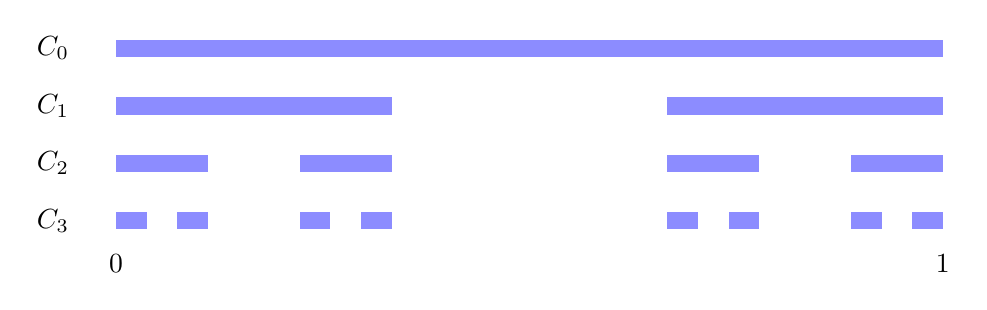
\begin{tikzpicture}[x=10.5cm,y=0.73cm]
\foreach \y/\lab in {0/{$C_0$},1/{$C_1$},2/{$C_2$},3/{$C_3$}} {
  \node[anchor=east] at (-0.045,-\y) {\lab};
}
\fill[blue!45] (0,-0.15) rectangle (1,0.15);
\foreach \a/\b in {0/0.333333,0.666667/1} {
  \fill[blue!45] (\a,-1.15) rectangle (\b,-0.85);
}
\foreach \a/\b in {0/0.111111,0.222222/0.333333,0.666667/0.777778,0.888889/1} {
  \fill[blue!45] (\a,-2.15) rectangle (\b,-1.85);
}
\foreach \a/\b in {0/0.037037,0.074074/0.111111,0.222222/0.259259,0.296296/0.333333,0.666667/0.703704,0.740741/0.777778,0.888889/0.925926,0.962963/1} {
  \fill[blue!45] (\a,-3.15) rectangle (\b,-2.85);
}
\node[anchor=north] at (0,-3.42) {$0$};
\node[anchor=north] at (1,-3.42) {$1$};
\end{tikzpicture}

\smallskip
\emph{Pierwsze cztery etapy konstrukcji środkowotrzeciego zbioru Cantora.
W każdym etapie pozostaje $2^n$ przedziałów długości $3^{-n}$.}
\end{center}

\begin{twierdzenie}[Podstawowe własności zbioru Cantora]
\label{thm:cantor-properties}
Zbiór Cantora $C\subseteq[0,1]$ jest niepusty, zwarty,
doskonały (zamknięty i bez punktów izolowanych),
nigdziegęsty (jego domknięcie ma puste wnętrze),
nieprzeliczalny i ma miarę Lebesgue'a zero.
Co więcej, jest w naturalny sposób homeomorficzny
z przestrzenią $\{0,1\}^{\mathbb N}$ wyposażoną
w topologię produktową. W tym przypadku topologia ta
jest generowana przez cylindry, czyli zbiory wszystkich
ciągów zero-jedynkowych o ustalonych pierwszych
$N$ wyrazach, dla dowolnego $N\ge1$.
\end{twierdzenie}

\begin{proof}
Każdy $C_n$ jest niepusty i zwarty, a zbiory są
malejące. Ich przekrój jest więc niepusty i zwarty.
Zbiór $C_n$ jest sumą $2^n$ domkniętych przedziałów
długości $3^{-n}$. Końce tych przedziałów należą do
$C$, ponieważ w dalszych etapach usuwamy wyłącznie
otwarte przedziały środkowe. Dla dowolnego $x\in C$
możemy znaleźć w dowolnie małym otoczeniu $x$
inny koniec przedziału składowego $C_n$.
Stąd $C$ nie ma punktów izolowanych.

Każdy przedział składowy $C_n$ ma długość $3^{-n}$.
Gdyby $C$ zawierał przedział otwarty dodatniej długości,
to musiałby on być zawarty w jednym z przedziałów
składowych każdego $C_n$, co jest niemożliwe dla
dostatecznie dużego $n$. Zatem wnętrze $C$ jest puste;
ponieważ $C$ jest zamknięty, jest nigdziegęsty.

Z monotoniczności miary i skończonej addytywności
otrzymujemy
$0\le\lambda_1(C)\le\lambda_1(C_n)=2^n3^{-n}=(2/3)^n$.
Przechodząc do granicy, dostajemy $\lambda_1(C)=0$.

Na każdym etapie wybrana przez punkt $x\in C$ lewa lub prawa
trzecia część przedziału wyznacza odpowiednio cyfrę $0$ lub $2$.
Długości przedziałów maleją do zera, a ich zagnieżdżenie
ma dokładnie jeden punkt wspólny. Zatem punkt $x\in C$
ma przedstawienie trójkowe
$x=\sum_{n\ge1}2\varepsilon_n3^{-n}$, gdzie
$\varepsilon_n\in\{0,1\}$. W obrębie cyfr $0$ i $2$
to przedstawienie jest jednoznaczne: jeżeli ciągi
różnią się po raz pierwszy na miejscu $k$, to różnica
składników z tego miejsca to $2\cdot3^{-k}$,
a możliwa suma różnic z późniejszych miejsc ma wartość
bezwzględną co najwyżej
$\sum_{n>k}2\cdot3^{-n}=3^{-k}$.
Odwzorowanie
$\Phi:\{0,1\}^{\mathbb N}\to C$ dane przez
$\Phi((\varepsilon_n))=\sum_n2\varepsilon_n3^{-n}$
jest więc bijekcją. Jeśli dwa ciągi mają pierwszych
$N$ cyfr jednakowych, ich obrazy różnią się o co
najwyżej $\sum_{n>N}2\cdot3^{-n}=3^{-N}$;
to dowodzi ciągłości $\Phi$ dla topologii produktowej.
Dziedzina jest zwarta. Można to stwierdzić bez użycia
twierdzenia Tychonoffa: metryka
$\rho(u,v)=\sum_{n\ge1}2^{-n}|u_n-v_n|$
wyznacza tę samą topologię co cylindry; z każdego ciągu
punktów można wybrać podciąg o stałej pierwszej
współrzędnej, następnie jego podciąg o stałej drugiej
współrzędnej itd. Przekątniowy podciąg jest zbieżny
w metryce $\rho$, co dowodzi zwartości metrycznej.
Ponieważ $C$ jest przestrzenią Hausdorffa,
ciągła bijekcja ze zwartej dziedziny jest homeomorfizmem.
Ponieważ $\{0,1\}^{\mathbb N}$ jest nieprzeliczalna,
tak samo jest z $C$.
\end{proof}

\begin{wniosek}[Lebesgue'owskie zbiory nieborelowskie]
\label{cor:nonborel-lebesgue}
Istnieją podzbiory $\mathbb R$ mierzalne w sensie
Lebesgue'a, które nie są borelowskie. W szczególności
$\mathcal B(\mathbb R)\subsetneq\mathcal L_1$.
\end{wniosek}

\begin{proof}
Zbiór Cantora $C$ jest borelowski, ma miarę zero
i ma moc continuum $\mathfrak c$.
Każdy jego podzbiór jest mierzalny w sensie Lebesgue'a,
ponieważ miara $\lambda_1$ jest zupełna.
Rodzina wszystkich podzbiorów $C$ ma moc
$2^{\mathfrak c}>\mathfrak c$ (twierdzenie Cantora),
podczas gdy rodzina zbiorów borelowskich prostej ma
moc co najwyżej $\mathfrak c$. Uzasadnijmy ostatnie
stwierdzenie. Rodzina przedziałów o końcach wymiernych
jest przeliczalną bazą topologii $\mathbb R$. Każdy
zbiór borelowski można opisać za pomocą
\emph{przeliczalnego kodu borelowskiego}: dobrze
ufundowanego drzewa, którego węzły są oznaczone
operacją dopełnienia, sumy przeliczalnej albo
jednym z przedziałów bazowych. Takie opisy otrzymuje
się indukcyjnie po etapach tworzenia najmniejszej
rodziny zamkniętej na dopełnienia i sumy przeliczalne.
Każde drzewo o przeliczalnie wielu węzłach jest
kodowane przez podzbiór zbioru wszystkich skończonych
ciągów liczb naturalnych wraz z przeliczalnym
etykietowaniem. Liczba takich kodów wynosi co najwyżej
$2^{\aleph_0}=\mathfrak c$. Wynika stąd, że zbiorów
borelowskich jest najwyżej $\mathfrak c$, zaś
podzbiorów $C$ jest $2^{\mathfrak c}$; na mocy
twierdzenia Cantora $2^{\mathfrak c}>\mathfrak c$.
Zatem nie każdy podzbiór $C$ jest borelowski.
\end{proof}

\section{Zbiór dodatniej miary bez wnętrza}

\begin{przyklad}[Zbiór Smitha--Volterry--Cantora]
\label{ex:fat-cantor}
Rozpoczynamy od $F_0=[0,1]$. Na etapie $n\ge1$
z każdego z $2^{n-1}$ przedziałów pozostawionych
w poprzednim etapie usuwamy otwarty przedział środkowy
długości $4^{-n}$; pozostały zbiór oznaczamy $F_n$.
Można to wykonać na każdym etapie: długość każdego
z dwóch potomnych przedziałów jest dodatnia.
W rzeczy samej, jeśli $\ell_n$ oznacza długość jednego
przedziału składowego $F_n$, to
$\ell_0=1$ i $\ell_n=(\ell_{n-1}-4^{-n})/2$.
Indukcja daje dokładny wzór
$\ell_n=2^{-n-1}+2^{-2n-1}>0$; co więcej,
$\ell_{n-1}>4^{-n}$, a zatem każde kolejne
usunięcie jest geometrycznie możliwe.

Łączna długość usuniętych przedziałów na etapie $n$
wynosi $2^{n-1}4^{-n}=2^{-n-1}$. Ponieważ otwarte
przedziały usuwane w różnych etapach są rozłączne,
dla $F=\bigcap_nF_n$ mamy
\[
\lambda_1(F)=1-\sum_{n=1}^\infty2^{-n-1}=\frac12.
\]
Zbiór $F$ jest zwarty. Ponieważ długości przedziałów
składowych $F_n$ dążą do zera, $F$ nie zawiera
niepustego przedziału otwartego, jest więc nigdziegęsty.
Końce każdego przedziału składowego pozostają w $F$,
a zatem, podobnie jak dla zbioru Cantora, żaden punkt
$F$ nie jest izolowany. Zbiór $F$ jest więc doskonały
i ma dodatnią miarę. A zatem nawet jednoczesna
zwartość, brak wnętrza i nigdziegęstość nie
wymuszają miary zero.
\end{przyklad}

\section{Funkcja Cantora i miara osobliwa: zapowiedź}

\begin{przyklad}[Funkcja Cantora]
\label{ex:cantor-function}
Dla $x\in C$ o przedstawieniu
$x=\sum_{n\ge1}2\varepsilon_n3^{-n}$ określamy
$F(x)=\sum_{n\ge1}\varepsilon_n2^{-n}$.
Na każdej składowej otwartej $[0,1]\setminus C$
przedłużamy $F$ jako funkcję stałą, przyjmując
wspólną wartość na końcach tej składowej.
Wartości końcowe są równe: końce przedziału
usuniętego na etapie $n$ mają przedstawienia
trójkowe, których pierwsze $n-1$ cyfr są jednakowe,
a pozostałe cyfry są odpowiednio $0,2,2,\ldots$
oraz $2,0,0,\ldots$, co w dwójkowym zapisie
prowadzi do tej samej liczby.

Tak uzyskana funkcja $F:[0,1]\to[0,1]$
jest ciągła i niemalejąca. Można to sprawdzić za
pomocą kolejnych ciągłych przybliżeń $F_n$:
na każdym przedziale składowym $C_n$ funkcja $F_n$
jest liniowa, a na przedziałach już usuniętych
stała, przy czym $F_n(0)=0$ oraz $F_n(1)=1$.
Dokładniej: na każdym z $2^n$ domkniętych przedziałów
składowych $C_n$ wartości na końcach różnią się o
$2^{-n}$, a na przedziałach już usuniętych $F_n$
pozostaje stała. Z konstrukcji wynika, że
$\|F_{n+1}-F_n\|_\infty\le 2^{-n}$.
Dla $m>n$ dostajemy
$\|F_m-F_n\|_\infty\le\sum_{k=n}^{m-1}2^{-k}$,
więc $(F_n)$ jest jednostajnym ciągiem Cauchy'ego.
Jego granica jest ciągła i niemalejąca. Na końcach
każdego usuniętego przedziału granica przyjmuje
wspólną, raz ustaloną wartość, a na $C$ zgadza się
z szeregiem definiującym $F$, ponieważ na przedziale
składowym $C_n$ zarówno $F_n$, jak i wartość tego
szeregu leżą między tymi samymi wartościami końcowymi,
oddalonymi o $2^{-n}$. To identyfikuje granicę
jednostajną z funkcją $F$ z definicji.

Ponadto $F$ jest stała na każdym przedziale
składowym $[0,1]\setminus C$, więc $F'(x)=0$
dla wszystkich $x\in(0,1)\setminus C$.
Ponieważ $\lambda_1(C)=0$, mamy $F'=0$
prawie wszędzie, ale $F(1)-F(0)=1$.
Nie jest to sprzeczność: funkcja Cantora nie jest
absolutnie ciągła. Przypomnijmy, że funkcja
$h:[a,b]\to\mathbb R$ jest absolutnie ciągła, jeśli
dla każdego $\varepsilon>0$ istnieje $\delta>0$
takie, że dla każdej skończonej rodziny parami
rozłącznych przedziałów $(a_k,b_k)\subseteq[a,b]$
warunek $\sum_k(b_k-a_k)<\delta$ implikuje
$\sum_k|h(b_k)-h(a_k)|<\varepsilon$.
Dla funkcji Cantora bierzemy $2^n$ przedziałów
składowych $C_n$. Suma ich długości wynosi
$(2/3)^n\to0$, podczas gdy suma przyrostów $F$
na tych przedziałach wynosi
$2^n\cdot2^{-n}=1$. Sprzeczność z powyższą definicją
dla $\varepsilon=1/2$ dowodzi braku absolutnej ciągłości.
W rozdziałach o całce Lebesgue'a i rozkładzie miar
zobaczymy, że $F$ wyznacza bezatomową miarę
osobliwą względem miary Lebesgue'a, to znaczy
skoncentrowaną na zbiorze o mierze Lebesgue'a zero.
\end{przyklad}

\section{Zbiór Vitaliego i ograniczenia mierzalności}

\begin{twierdzenie}[Istnienie zbioru niemierzalnego]
\label{thm:vitali}
Przy aksjomacie wyboru istnieje podzbiór
$V\subseteq[0,1]$, który nie jest mierzalny
w sensie Lebesgue'a.
\end{twierdzenie}

\begin{proof}
Na $[0,1]$ wprowadzamy relację równoważności
$x\sim y$ wtedy i tylko wtedy, gdy $x-y\in\mathbb Q$.
Z każdej klasy wybieramy dokładnie jeden element,
tworząc zbiór reprezentantów $V\subseteq[0,1]$.
Ten krok wykorzystuje aksjomat wyboru.

Niech $Q=\mathbb Q\cap[-1,1]$. Zbiory $V+q$ dla
$q\in Q$ są parami rozłączne. Rzeczywiście, gdyby
$v_1+q_1=v_2+q_2$, to
$v_1-v_2=q_2-q_1\in\mathbb Q$, więc $v_1,v_2$
należałyby do tej samej klasy; wybór reprezentantów
daje $v_1=v_2$ i następnie $q_1=q_2$.

Mamy też
\begin{equation}\label{eq:vitali-sandwich}
[0,1]\subseteq\bigcup_{q\in Q}(V+q)\subseteq[-1,2].
\end{equation}
Pierwsze zawieranie wynika stąd, że dla dowolnego
$x\in[0,1]$ istnieje $v\in V$ z $x-v\in\mathbb Q$,
a jednocześnie $|x-v|\le1$.

Przypuśćmy, że $V$ jest mierzalny. Z niezmienniczości
translacyjnej $\lambda_1(V+q)=\lambda_1(V)$.
Zbiory $V+q$ są rozłączne, $Q$ jest przeliczalny i
nieskończony, a więc
\[
\lambda_1\Big(\bigcup_{q\in Q}(V+q)\Big)
=\sum_{q\in Q}\lambda_1(V)
=\begin{cases}0,&\lambda_1(V)=0,\\
\infty,&\lambda_1(V)>0.
\end{cases}
\]
Z \eqref{eq:vitali-sandwich} wynika jednak, że lewa
strona znajduje się między $1$ a $3$. To sprzeczność.
Zatem $V\notin\mathcal L_1$.
\end{proof}

\begin{wniosek}[Nie istnieje miara długości wszystkich podzbiorów]
\label{cor:no-all-subsets-invariant}
Nie istnieje przeliczalnie addytywna miara
$\nu:\mathcal P(\mathbb R)\to[0,\infty]$, która
jest niezmiennicza względem translacji i spełnia
$\nu([0,1])=1$.
\end{wniosek}

\begin{proof}
Najpierw musimy ustalić $\nu(\{0\})=0$.
Gdyby $\nu(\{0\})>0$, przeliczalnie wiele
rozłącznych translacji singletonu zawartych w $[0,1]$
miałoby miarę nieskończoną, sprzecznie z
$\nu([0,1])=1$. Zatem $\nu(\{0\})=0$,
a translacyjna niezmienniczość daje
$\nu(\{x\})=0$ dla każdego $x\in\mathbb R$.
Wobec tego $\nu([0,1))=\nu([0,1])=1$.
Trzy rozłączne przedziały $[-1,0)$, $[0,1)$
i $[1,2)$ mają po jednej jednostce miary;
po dodaniu punktu $2$ otrzymujemy
$\nu([-1,2])=3$. Teraz dowód Vitaliego stosuje się
bez zmian do $\nu$, ponieważ wszystkie podzbiory
w nim występujące należałyby do dziedziny $\nu$.
Otrzymujemy sprzeczność.
\end{proof}

\begin{uwaga}[Precyzyjny sens niemożliwości]
Powyższe twierdzenie nie zabrania istnienia miar na
$\mathcal P(\mathbb R)$, takich jak miara licząca
czy miara zerowa. Stwierdza niemożliwość jednoczesnego
zachowania \emph{przeliczalnej addytywności},
\emph{niezmienniczości translacyjnej} i
\emph{normalizacji długości przedziału}.
\end{uwaga}

\section{Podsumowanie i przygotowanie do całki}

Wykazaliśmy, że objętość prostopadłościanów
półotwartych wyznacza jedną miarę borelowską,
której uzupełnieniem jest miara Lebesgue'a. Zbiory
mierzalne mają aproksymacje otwarte i zwarte.
Gęstość, nigdziegęstość czy nieprzeliczalność
nie przesądzają o wielkości miary zbioru.

W następnych rozdziałach zdefiniujemy funkcje
mierzalne i całkę oraz wyjaśnimy rolę absolutnej
ciągłości w związku między całką a pochodną.